\documentclass[11pt, a4paper]{article}
\usepackage[utf8]{inputenc}
\usepackage[T1]{fontenc}
\usepackage[portuguese]{babel}
\usepackage{graphicx}
\usepackage{float}
\usepackage{geometry}
\usepackage{amsmath}
\usepackage{listings}
\usepackage[table]{xcolor}
\usepackage{pdfpages}

% Configuração das Margens
\geometry{top=2.5cm, bottom=2.5cm, left=3cm, right=3cm}

% Configuração de Cores para o Código
\definecolor{codegreen}{rgb}{0,0.6,0}
\definecolor{codegray}{rgb}{0.5,0.5,0.5}
\definecolor{codepurple}{rgb}{0.58,0,0.82}
\definecolor{backcolour}{rgb}{0.95,0.95,0.92}

\lstdefinestyle{mystyle}{
    backgroundcolor=\color{backcolour},
    commentstyle=\color{codegreen},
    keywordstyle=\color{magenta},
    numberstyle=\tiny\color{codegray},
    stringstyle=\color{codepurple},
    basicstyle=\ttfamily\footnotesize,
    breakatwhitespace=false,
    breaklines=true,
    captionpos=b,
    keepspaces=true,
    numbers=left,
    numbersep=5pt,
    showspaces=false,
    showstringspaces=false,
    showtabs=false,
    tabsize=2
}
\lstset{style=mystyle}

\begin{document}

% --- CAPA ---
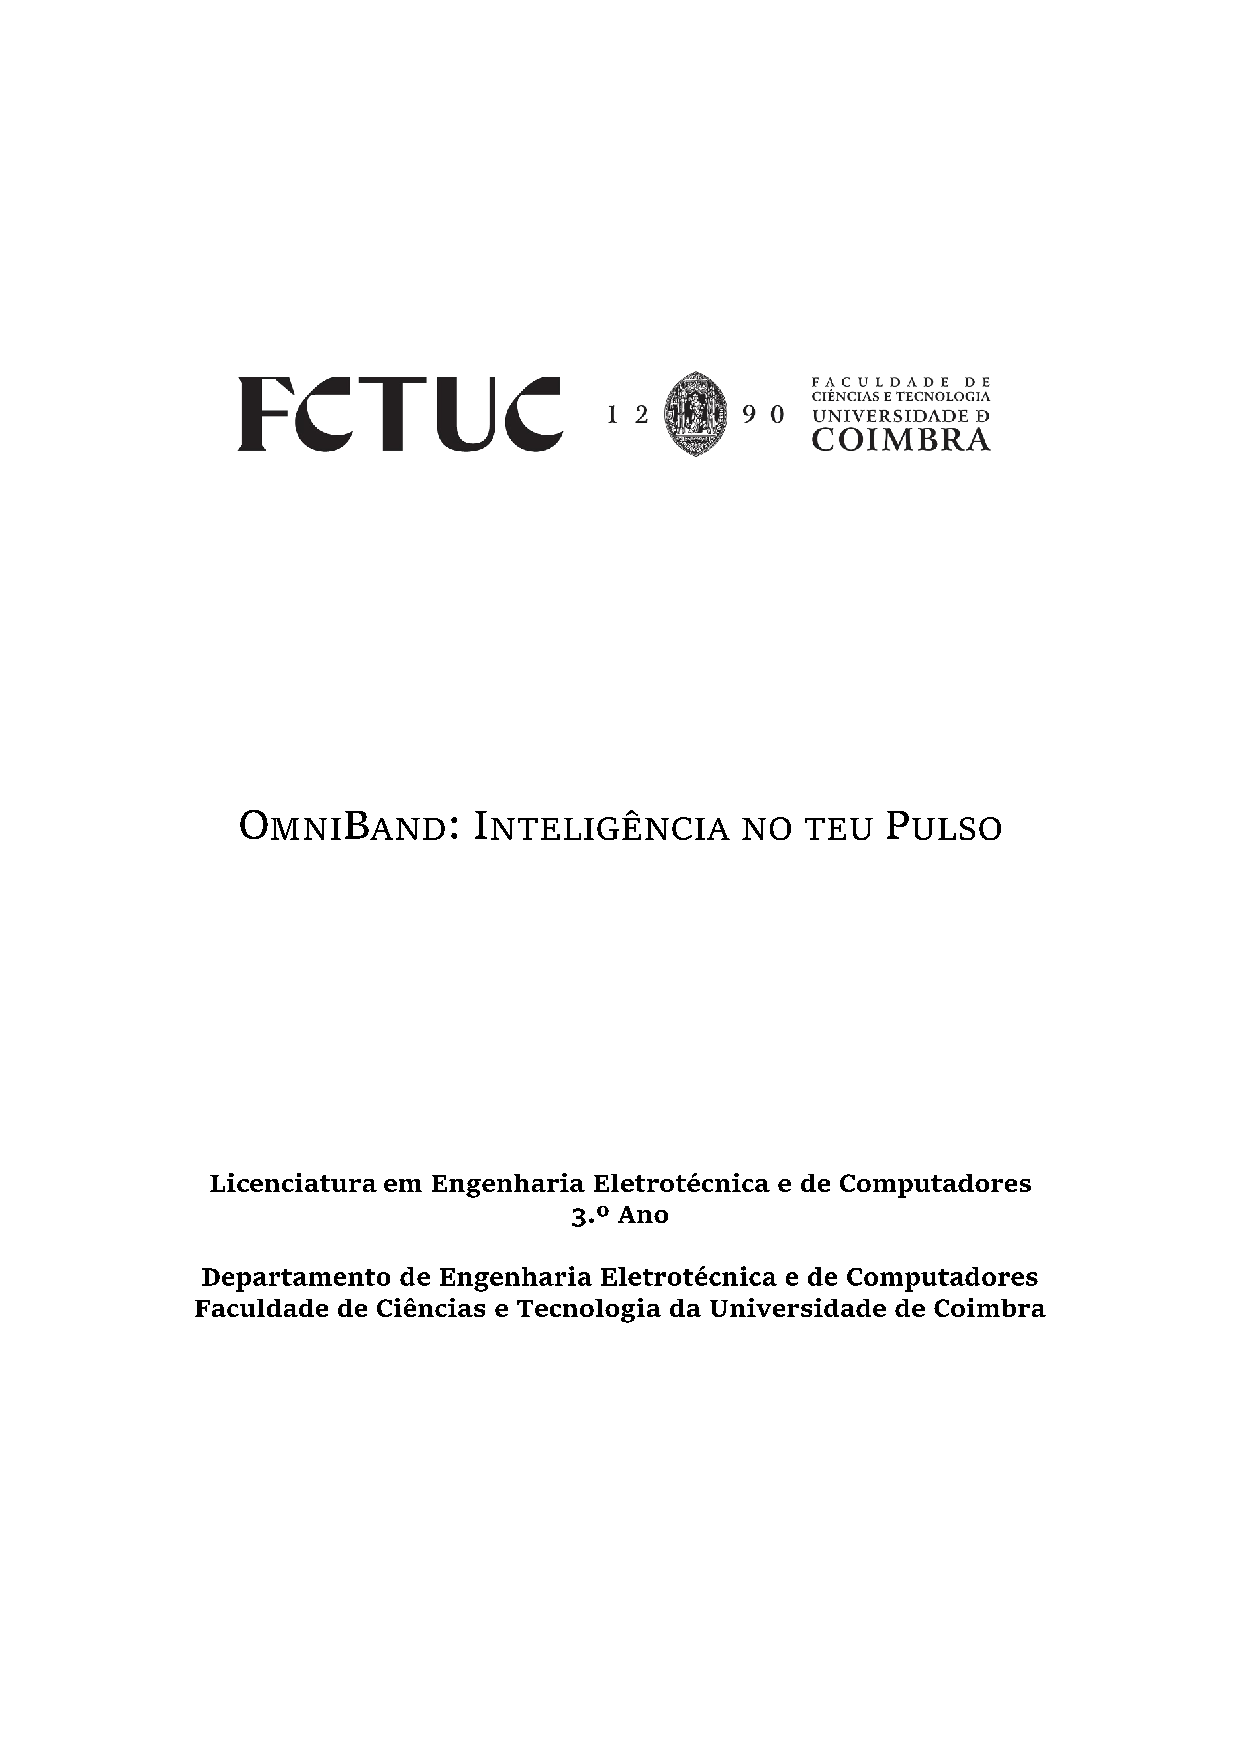
\includepdf[pages={1}]{capa3.pdf}

\tableofcontents
\newpage

\section*{OmniBand: Inteligência no teu pulso}

\begin{abstract}
    O OmniBand é um wearable IoT de baixo consumo, assente em TinyML, pensado para automação residencial. O conceito original — uma ``varinha mágica'' no pulso combinando voz (contexto) e gesto (ação) com processamento local — foi adaptado ao longo do projeto devido a condicionantes logísticas. Todos os materiais chegaram tardiamente e o microcontrolador planeado (M5StickC Plus2) nunca esteve disponível. A equipa pivotou para o M5CoreInk (único hardware disponível), substituindo a seleção de contexto por voz por um sistema de deteção de palmas (1, 2 ou 3 palmas) e o backend cloud por um servidor local Flask integrado com Home Assistant. O resultado é um protótipo funcional que demonstra controlo residencial por gestos com Machine Learning na periferia (Edge Impulse), comunicação Wi-Fi e um dashboard web em tempo real.
\end{abstract}

\begin{table}[H]
    \small
    \begin{tabular}{|p{0.3\textwidth}|p{0.45\textwidth}|}
        \hline
        \cellcolor{lightgray}\textbf{Contacto principal:} & Gonçalo Peres \\
        \hline
    \end{tabular}
\end{table}

\begin{table}[H]
    \small
    \begin{tabular}{|p{0.35\textwidth}|p{0.2\textwidth}|}
        \hline
        \cellcolor{lightgray}\textbf{Data de início:} & Fevereiro de 2026 \\
        \hline
        \cellcolor{lightgray}\textbf{Data de conclusão:} & Junho de 2026 \\
        \hline
        \cellcolor{lightgray}\textbf{Duração (meses):} & 5 meses \\
        \hline
    \end{tabular}
\end{table}

\textbf{Lista de participantes}

\begin{table}[H]
    \small
    \centering
    \begin{tabular}{|p{0.05\textwidth}|p{0.20\textwidth}|p{0.15\textwidth}|p{0.31\textwidth}|p{0.14\textwidth}|}
        \hline
        \cellcolor{lightgray}\textbf{N.º} &
        \cellcolor{lightgray}\textbf{Nome} &
        \cellcolor{lightgray}\textbf{Nº Aluno} &
        \cellcolor{lightgray}\textbf{E-mail contacto} &
        \cellcolor{lightgray}\textbf{Turma PL} \\
        \hline
        1 & Diogo Correia & 2023215978 & diogolopescorreia28@gmail.com & PL2 \\
        \hline
        2 & Diogo Flórido & 2020233528 & diogo.florido@student.uc.pt & PL2 \\
        \hline
        3 & Gonçalo Peres & 2023212120 & goncaloperes02@gmail.com & PL2 \\
        \hline
        4 & Gustavo Dias & 2023212954 & gustavogaspardias@gmail.com & PL2 \\
        \hline
    \end{tabular}
\end{table}

\section{Descrição do projeto com identificação dos objetivos e metas}

\subsection{Descrição do problema}
Hoje, a automação residencial é dominada por duas vias: apps no smartphone e assistentes de voz na cloud (ex., Amazon Alexa, Google Assistant). Ambas introduzem fricção na experiência. As apps obrigam a parar o que se está a fazer para ``mexer no ecrã'', e os assistentes de voz dependem de internet estável, trazendo latência e questões de privacidade. Além disso, não são práticos para comandos ``analógicos'' (por exemplo, dizer ``coloca a luz a 73\%''). Faz falta uma interface humano-máquina mais natural, rápida e que não dependa da cloud para o processamento principal. O desafio é criar um wearable capaz de interpretar intenções (contexto + ação) em tempo real, com baixo consumo energético e com os dados a serem tratados localmente.

\subsection{Objetivos}
O projeto tem como meta desenvolver o OmniBand, um protótipo funcional de uma interface wearable multimodal baseada no conceito de ``varinha mágica''. Os objetivos específicos são:
\begin{itemize}
    \item \textbf{Hardware e Integração:} Implementar o sistema num microcontrolador de baixo custo e baixo consumo (M5CoreInk), utilizando sensores externos (IMU BMI088 e microfone analógico);
    \item \textbf{Machine Learning (Edge AI):} Treinar e implementar modelos de TinyML localmente (Edge Impulse) para reconhecimento de gestos (cima, baixo, parado);
    \item \textbf{Eficiência Energética:} Desenvolver uma máquina de estados assimétrica, onde o IMU atua como gatilho (``raise-to-wake'') para ativar o microfone, evitando a amostragem contínua de áudio;
    \item \textbf{Comunicação e Backend:} Estabelecer comunicação sem fios via Wi-Fi, sincronizando o estado dos dispositivos com um servidor local (Flask + Home Assistant);
    \item \textbf{Interface Complementar:} Desenvolver um Dashboard Web que permita a visualização de estados e controlo das ações da pulseira.
\end{itemize}

\subsection{Adaptações ao longo do projeto}
O percurso de desenvolvimento do OmniBand foi fortemente condicionado por fatores logísticos alheios à equipa. O microcontrolador inicialmente planeado, o \textbf{M5StickC Plus2}, nunca esteve disponível durante todo o semestre. Todos os materiais didáticos e de prototipagem chegaram com atrasos significativos, tendo a equipa acesso apenas ao hardware que já se encontrava na posse do laboratório.

A solução encontrada foi pivotar para o \textbf{M5CoreInk}, o único dispositivo disponível. Esta mudança forçou várias adaptações na arquitetura do sistema:

\begin{itemize}
    \item \textbf{Ecrã:} O M5CoreInk possui um ecrã de tinta eletrónica (e-paper) de 200$\times$200 pixels, de atualização lenta, exigindo uma interface de utilizador otimizada (modos de atualização rápida/lenta, desenho incremental com clip rects);
    \item \textbf{Sensores:} O M5CoreInk não tem IMU nem microfone integrados. A equipa integrou um \textbf{BMI088} externo (acelerómetro + giroscópio) via I2C e um microfone eletreto analógico básico;
    \item \textbf{Microfone:} O microfone disponível era um eletreto analógico simples, incapaz de captar voz inteligível. A seleção de contexto por comando de voz foi substituída por um sistema de \textbf{deteção de palmas} (1 palma = corredor, 2 = sala, 3 = quarto);
    \item \textbf{Backend:} A cloud Firebase foi substituída por um \textbf{servidor Flask local} num Raspberry Pi, integrado com \textbf{Home Assistant} para controlo real de dispositivos smart home;
    \item \textbf{Interface:} A aplicação móvel foi substituída por um \textbf{Dashboard Web} com atualização em tempo real (polling a cada 2 segundos).
\end{itemize}

Estas adaptações demonstram a capacidade da equipa de responder a condicionantes reais de engenharia, mantendo a funcionalidade central do projeto: controlo residencial por gestos com processamento local de ML.

\subsection{Concept of Operations (ConOps)}
O OmniBand propõe uma experiência de utilizador fluida, onde o movimento é a ação principal e as palmas servem para selecionar o contexto/divisão.

\textbf{Ambiente Operacional}\\
O sistema opera dentro do ecossistema de uma habitação inteligente (Smart Home). Os dispositivos controlados (lâmpadas, tomadas) encontram-se distribuídos por várias divisões e partilham a mesma infraestrutura de rede local.

\textbf{Elementos Principais do Sistema}
\begin{itemize}
    \item \textbf{Wearable (OmniBand):} Dispositivo de pulso (M5CoreInk) que atua como o principal meio de aquisição (IMU BMI088 e microfone analógico) e processamento (algoritmos TinyML no Edge) de dados.
    \item \textbf{Servidor Central:} Raspberry Pi com servidor Flask e Home Assistant, responsável por traduzir os comandos recebidos da pulseira em instruções para os periféricos.
    \item \textbf{Web Dashboard:} Interface gráfica para configuração de gestos, dispositivos, regras e monitorização em tempo real.
    \item \textbf{Atuadores Físicos:} Equipamentos IoT comerciais (ex: smart plugs Tapo P110).
\end{itemize}

\textbf{Interfaces Externas}\\
A comunicação primária entre o wearable e o servidor central é feita via \textbf{Wi-Fi}. O dispositivo possui um ecrã e-paper para fornecer feedback visual instantâneo (validação de comandos, estado do sistema). O dashboard web permite controlo adicional e personalização.

\textbf{Cenário de Utilização (Use Scenario)}\\
O utilizador chega a casa com sacos de compras nas mãos e o corredor está escuro. Em vez de pousar os sacos para tirar o telemóvel do bolso, move o pulso para ativar o OmniBand. Dá \textbf{1 palma} para selecionar o contexto ``corredor''. De seguida, executa um gesto de rodar o pulso para cima. O modelo de Machine Learning no OmniBand reconhece o gesto ``Cima'' e emite imediatamente o comando via Wi-Fi para o servidor Flask, que aciona a lâmpada do corredor através do Home Assistant. A interação demorou menos de dois segundos, exigiu zero toque em ecrãs e a tarefa principal do utilizador (carregar as compras) não foi interrompida.

\subsection{Objetivos do Projeto face ao Estado da Arte}
No mercado, o controlo residencial continua dominado por soluções Cloud-AI (voz processada em servidores remotos) ou por wearables de alto custo (ex.: gestos no Apple Watch). O contributo do OmniBand é trazer esta lógica para dispositivos acessíveis, usando TinyML para correr modelos no microcontrolador, com limitações reais de memória e energia, e demonstrando que é possível construir um sistema funcional mesmo com hardware limitado e condicionantes logísticas.

\section{Capacidade de execução}
\subsection{Estrutura e lógica do plano de trabalho}
O plano de trabalhos segue uma lógica iterativa, adequada à prototipagem de IoT e ML. Depois da fase de requisitos, o projeto avançou em três frentes paralelas:
\begin{enumerate}
    \item Treino de modelos (Edge Impulse) — gestos cima, baixo, parado
    \item Firmware e comunicações — M5CoreInk + BMI088 + microfone + Wi-Fi
    \item Desenvolvimento do backend e dashboard — Flask + Home Assistant + Web UI
\end{enumerate}

Houve dependências claras: a comunicação para o servidor precisou de estar estável antes da integração do dashboard; em paralelo, a recolha de dados (IMU) foi essencial para treinar e colocar os modelos TinyML no microcontrolador. O atraso na entrega dos materiais comprimiu o cronograma, mas a equipa conseguiu entregar um protótipo funcional.

\subsection{Descrição e justificação do plano de investimentos}
O orçamento teve um teto de 300€ e focou-se em hardware Edge, atuadores para a demonstração final e materiais de prototipagem.

\begin{table}[H]
    \small
    \centering
    \begin{tabular}{|p{0.15\textwidth}|p{0.28\textwidth}|p{0.14\textwidth}|p{0.38\textwidth}|}
        \hline
        \cellcolor{lightgray}\textbf{Despesa} &
        \cellcolor{lightgray}\textbf{Descrição do Material} &
        \cellcolor{lightgray}\textbf{Custo Est.} &
        \cellcolor{lightgray}\textbf{Justificação} \\
        \hline
        Hardware Wearable & M5CoreInk + BMI088 + Microfone Eletreto & 35€ & Microcontrolador disponível (único acessível). IMU externo necessário pois o CoreInk não tem sensor inercial integrado. \\
        \hline
        Atuadores (Smart Home) & Tomadas Inteligentes Tapo P110 & 30€ & Necessários para validar visualmente a execução dos comandos de automação residencial. \\
        \hline
        Hardware Servidor & Raspberry Pi 4/5 + Cartão SD + Alimentação & 110€ & Servidor local para Flask, Home Assistant e base de dados SQLite. \\
        \hline
        Margem de Segurança & Portes de envio e componentes sobressalentes & 125€ & Fundo de reserva para substituição rápida de componentes. \\
        \hline
        \textbf{Total} & - & \textbf{300€} & - \\
        \hline
    \end{tabular}
\end{table}

\subsection{Identificação das atividades}
\begin{table}[H]
    \small
    \centering
    \begin{tabular}{|p{0.1\textwidth}|p{0.2\textwidth}|p{0.40\textwidth}|p{0.11\textwidth}|p{0.11\textwidth}|}
        \hline
        \cellcolor{lightgray}\textbf{Nº} &
        \cellcolor{lightgray}\textbf{Designação} &
        \cellcolor{lightgray}\textbf{Descrição} &
        \cellcolor{lightgray}\textbf{Início} &
        \cellcolor{lightgray}\textbf{Fim} \\
        \hline
        A1 & Engenharia de Requisitos & Definição do problema, arquitetura e conceitos. & 09/02/2026 & 29/03/2026 \\
        \hline
        A2 & Aquisição de Dados e Modelos ML & Gravação de datasets (IMU) e treino no Edge Impulse (3 classes: cima, baixo, parado). & 10/03/2026 & 25/04/2026 \\
        \hline
        A3 & Firmware e Integração IoT & Programação do M5CoreInk (C++) com BMI088, microfone, deteção de palmas, máquina de estados, e-paper UI. & 30/03/2026 & 15/05/2026 \\
        \hline
        A4 & Desenvolvimento Backend e Dashboard & Criação do servidor Flask, integração Home Assistant, Web Dashboard com polling em tempo real. & 15/04/2026 & 20/05/2026 \\
        \hline
        A5 & Testes de Sistema e Integração & Validação do fluxo completo: wake $\rightarrow$ palmas $\rightarrow$ gesto ML $\rightarrow$ servidor $\rightarrow$ atuador. & 06/04/2026 & 10/06/2026 \\
        \hline
        A6 & Preparação Final e Documentação & Redação do relatório, vídeo (pitch) e preparação do Demo Day. & 11/06/2026 & 25/06/2026 \\
        \hline
    \end{tabular}
\end{table}

\begin{figure}[H]
    \centering
    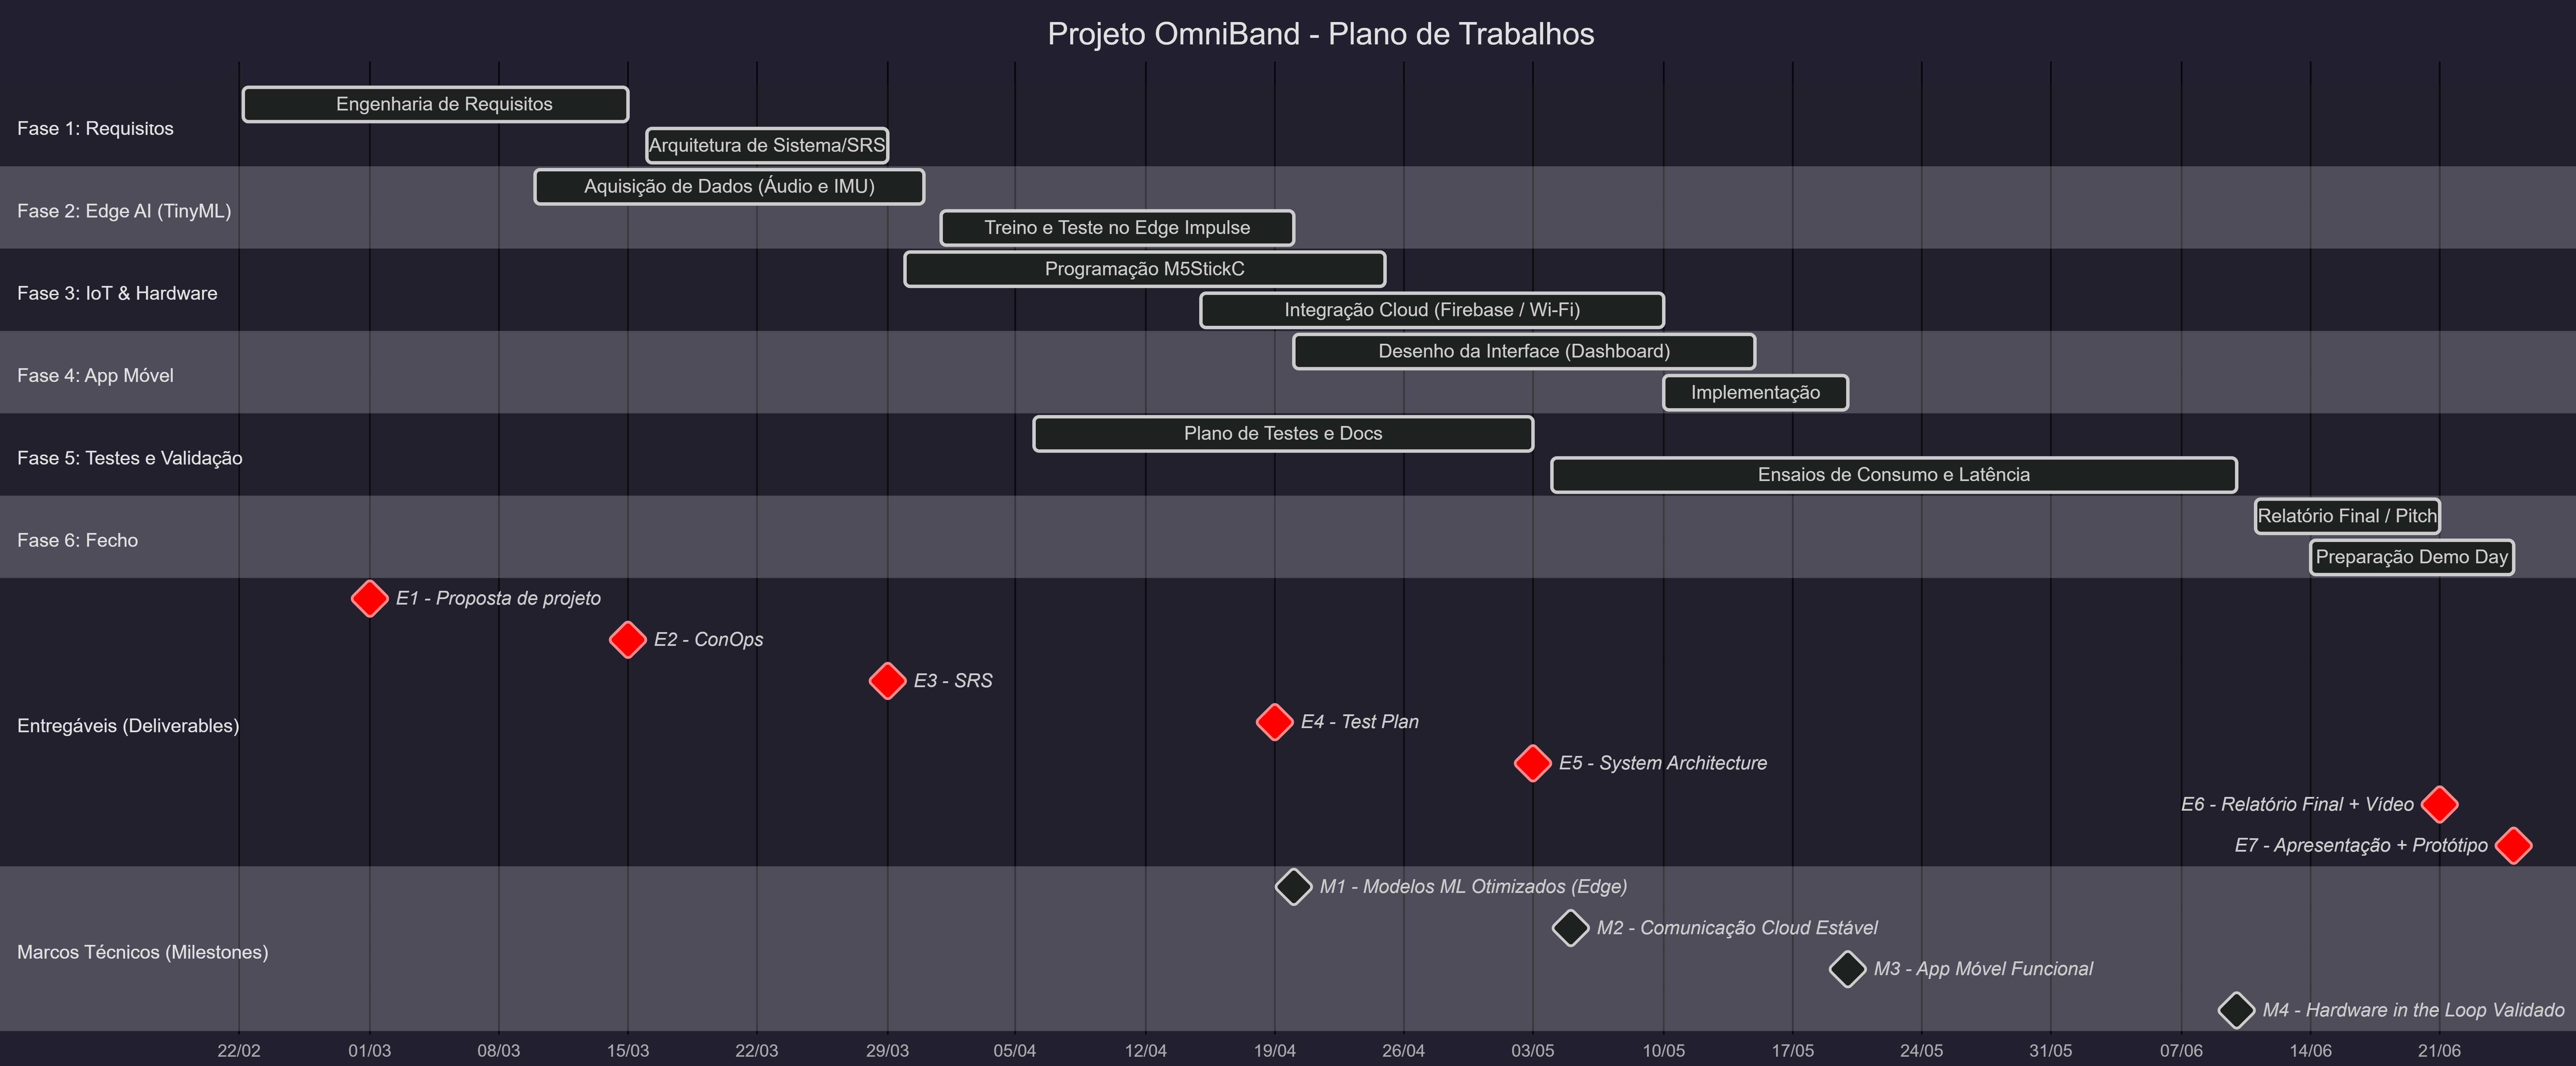
\includegraphics[width=1.06\textwidth]{Ganttv2.png}
    \caption{Gantt Chart}
\end{figure}

\subsection{Deliverables}
\begin{table}[H]
    \small
    \centering
    \begin{tabular}{|p{0.20\textwidth}|p{0.20\textwidth}|p{0.37\textwidth}|p{0.16\textwidth}|}
        \hline
        \cellcolor{lightgray}\textbf{Nº do Entregável} &
        \cellcolor{lightgray}\textbf{Nº da Atividade} &
        \cellcolor{lightgray}\textbf{Título do Entregável} &
        \cellcolor{lightgray}\textbf{Data Entrega} \\
        \hline
        E1 & A1 & Proposta de projecto & 01/03/2026 \\
        \hline
        E2 & A1 & ConOps & 15/03/2026 \\
        \hline
        E3 & A1 & SRS & 29/03/2026 \\
        \hline
        E4 & A5 & Test Plan & 19/04/2026 \\
        \hline
        E5 & A1, A3 & System Architecture & 03/05/2026 \\
        \hline
        E6 & A6 & Relatório Final + Vídeo & 21/06/2026 \\
        \hline
        E7 & A6 & Apresentação + Protótipo (Demo Day) & 25/06/2026 \\
        \hline
    \end{tabular}
\end{table}

\subsection{Milestones}
\begin{table}[H]
    \small
    \centering
    \begin{tabular}{|p{0.15\textwidth}|p{0.12\textwidth}|p{0.11\textwidth}|p{0.25\textwidth}|p{0.27\textwidth}|}
        \hline
        \cellcolor{lightgray}\textbf{Nº do Marco} &
        \cellcolor{lightgray}\textbf{Atividade} &
        \cellcolor{lightgray}\textbf{Entrega} &
        \cellcolor{lightgray}\textbf{Título} &
        \cellcolor{lightgray}\textbf{Meios de Verificação} \\
        \hline
        M1 & A2 & 20/04/2026 & Modelo ML Otimizado (Edge Impulse) & Avaliação das métricas de ML (acurácia cima/baixo/parado) \\
        \hline
        M2 & A3 & 05/05/2026 & Comunicação Wi-Fi Estável & Comando enviado do wearable refletido no servidor Flask \\
        \hline
        M3 & A4 & 20/05/2026 & Dashboard Web Funcional & Dashboard capaz de ler estados e controlar dispositivos \\
        \hline
        M4 & A5 & 10/06/2026 & Hardware in the Loop Validado & Protótipo executa o fluxo completo (palmas + gesto) sem bloqueios \\
        \hline
    \end{tabular}
\end{table}

\section{Especificação de Requisitos do Sistema (SRS)}

A análise e formulação dos requisitos foi desenvolvida seguindo o padrão estabelecido na norma ISO 29148. Devido às adaptações descritas na Secção 1.3, alguns requisitos foram revistos para refletir o hardware real (M5CoreInk em vez de M5StickC Plus2, deteção de palmas em vez de voz, servidor Flask em vez de Firebase).

\subsection{Necessidades dos Stakeholders (Needs)}
As necessidades fundamentais que orientam o desenvolvimento do OmniBand são:
\begin{itemize}
    \item \textbf{ND-001 Baixa Fricção de Interação:} O utilizador necessita de controlar dispositivos de automação residencial de forma rápida e intuitiva, sem depender exclusivamente de interações em ecrã ou de comandos de voz demorados.
    \item \textbf{ND-002 Privacidade e Autonomia:} O utilizador necessita de um sistema capaz de processar a maior parte da interação localmente, reduzindo a dependência de serviços cloud, a latência de resposta e os riscos associados à privacidade.
    \item \textbf{ND-003 Eficiência Energética:} O utilizador necessita de um wearable de baixo consumo energético, capaz de operar diariamente com minimização de processamento contínuo e de captação de áudio desnecessária.
\end{itemize}

\subsection{Rastreabilidade e Requisitos do Sistema}
A partir das necessidades descritas, foram derivados 10 requisitos de sistema (Funcionais e Não-Funcionais). A tabela seguinte apresenta a matriz de rastreabilidade resumida:

\begin{table}[H]
    \small
    \centering
    \begin{tabular}{|p{0.35\textwidth}|p{0.6\textwidth}|}
        \hline
        \cellcolor{lightgray}\textbf{Stakeholder Need (Origem)} &
        \cellcolor{lightgray}\textbf{Requisitos do Sistema Associados} \\
        \hline
        \textbf{ND-001} Baixa Fricção de Interação & SYS-FR-001, SYS-FR-003, SYS-FR-004, SYS-NFR-002, SYS-NFR-005 \\
        \hline
        \textbf{ND-002} Privacidade e Autonomia & SYS-FR-005, SYS-NFR-003, SYS-NFR-004 \\
        \hline
        \textbf{ND-003} Eficiência Energética & SYS-FR-002, SYS-NFR-001 \\
        \hline
    \end{tabular}
\end{table}

O detalhe técnico individual de cada requisito, bem como as ligações de mapeamento, encontram-se documentados no relatório gerado pelo Enterprise Architect, submetido em anexo (\textbf{projeto2\_e3.pdf}).

A Figura \ref{fig:traceability} apresenta a representação visual deste mapeamento.

\begin{figure}[H]
    \centering
    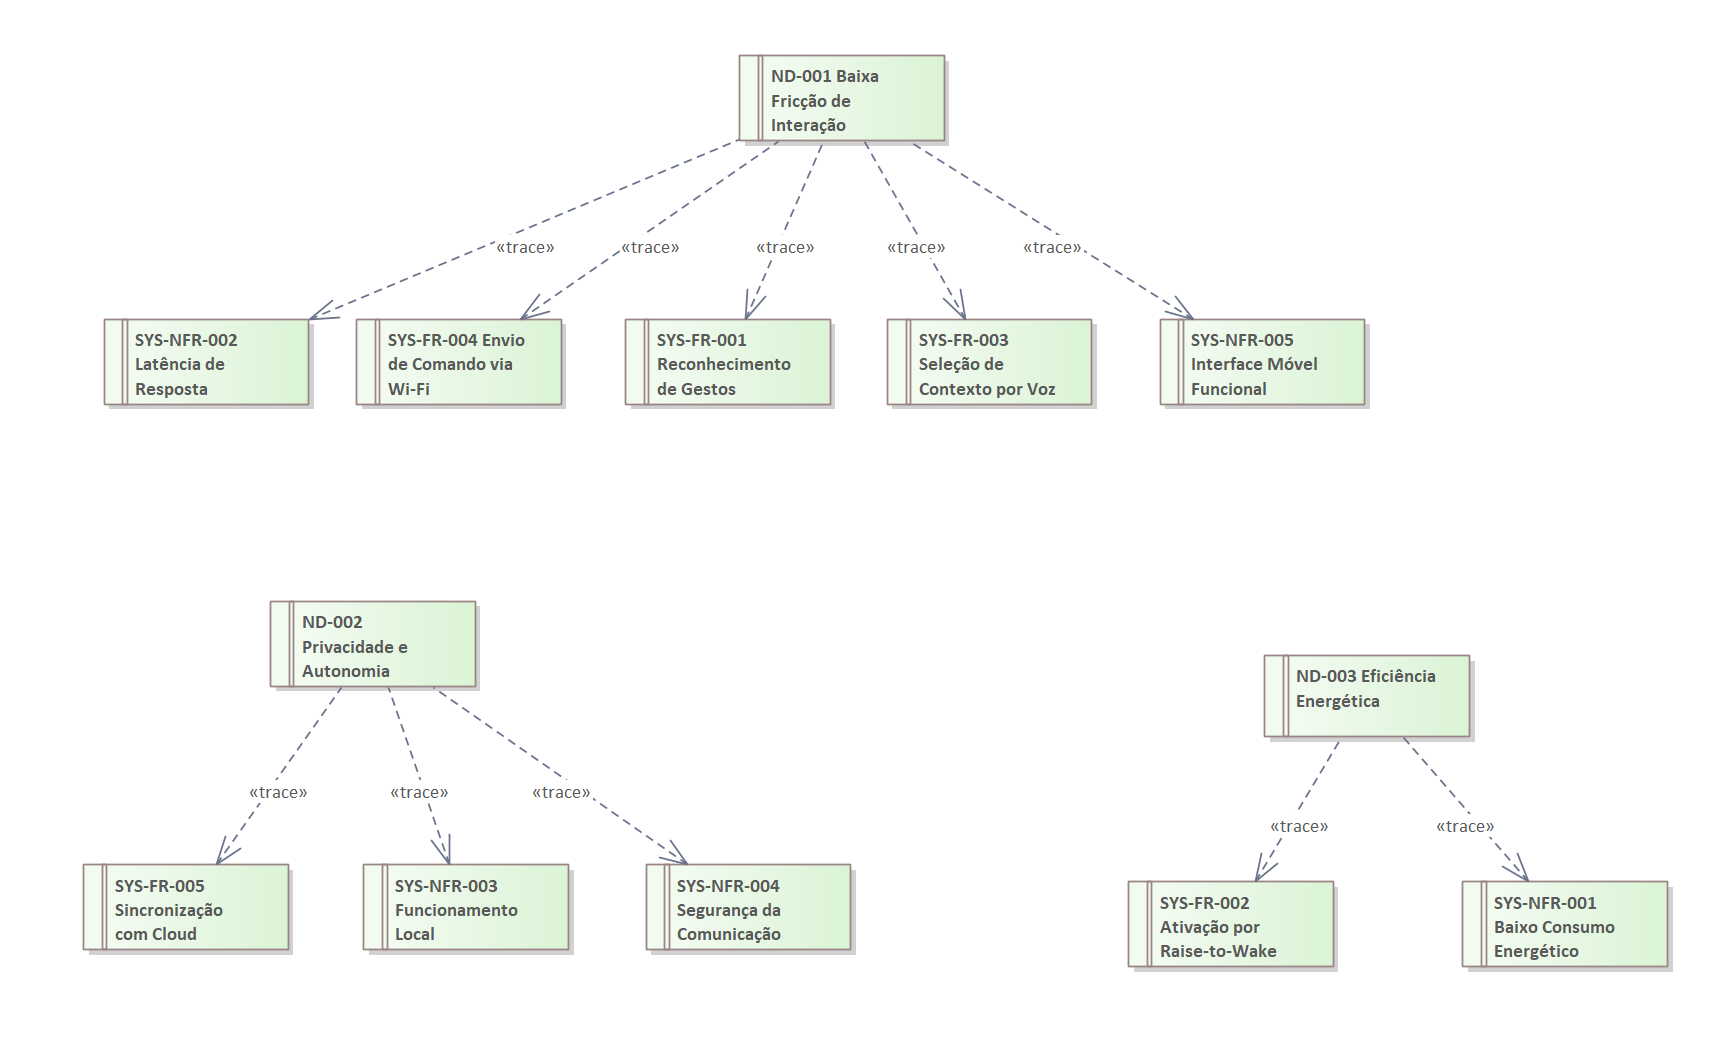
\includegraphics[width=0.95\textwidth]{traceability_diagram.png}
    \caption{Diagrama de Rastreabilidade (Stakeholder Needs vs. System Requirements)}
    \label{fig:traceability}
\end{figure}

\section{Verificação do Sistema (E4)}
\label{sec:verificacao_e4}

A Entrega E4 foca-se na Verificação do Sistema, demonstrando através de testes estruturados que a solução do projeto cumpre os Requisitos de Sistema (E3) definidos na fase anterior.

\subsection{Plano de Testes (ISO 29119-3)}

\subsubsection{Introdução e Itens a Testar}
O objetivo deste plano é definir a estratégia de verificação do sistema OmniBand, garantindo que o protótipo funcional cumpre as necessidades estabelecidas. Os testes focaram-se nos seguintes componentes:

\begin{itemize}
    \item O microcontrolador \textbf{M5CoreInk} (aquisição de dados do IMU BMI088 e microfone analógico, processamento Edge/TinyML, interface e-paper).
    \item A comunicação \textbf{Wi-Fi} e a sincronização de dados com o servidor Flask.
    \item A resposta dos \textbf{atuadores físicos} via Home Assistant (tomadas Tapo P110).
    \item O \textbf{Dashboard Web} com atualização em tempo real.
\end{itemize}

\subsubsection{Ambiente de Teste}
Os testes foram conduzidos num ambiente doméstico que simula a infraestrutura de uma rede local (Smart Home). O hardware de teste incluiu:
\begin{itemize}
    \item O wearable prototipado (M5CoreInk com bracelete, BMI088 externo, microfone eletreto).
    \item Um Raspberry Pi 4 a atuar como servidor local (Flask + Home Assistant).
    \item Tomadas Inteligentes Tapo P110 para verificação de resposta física.
\end{itemize}

\subsubsection{Estratégia}
A abordagem principal foi baseada em testes manuais do tipo Hardware-in-the-Loop (HIL). Os testes foram executados pelos membros da equipa simulando casos de uso reais. A estratégia consistiu em submeter o dispositivo a estímulos físicos (movimento do pulso para wake, palmas para contexto, gestos para ação). A verificação foi feita por observação direta do comportamento dos atuadores e validação cruzada do estado reportado no Dashboard Web.

\subsubsection{Critérios de Aprovação/Falha}
\begin{itemize}
    \item \textbf{Aprovação (Pass):} Um teste é considerado aprovado se o OmniBand processar a intenção localmente de forma correta, transmitir o comando com sucesso via Wi-Fi, e o atuador físico alterar o seu estado correspondente no tempo esperado, sem provocar a reinicialização ou bloqueio do sistema.
    \item \textbf{Falha (Fail):} O teste será considerado falhado se ocorrer um falso positivo/negativo no reconhecimento de gestos/palmas, se existirem perdas de comunicação que impeçam o acionamento, ou se for detetada uma falha na máquina de estados de gestão de energia.
\end{itemize}

\subsection{Protocolo de Testes e Rastreabilidade}

Abaixo apresentam-se as evidências de modelação extraídas do Enterprise Architect, detalhando o protocolo de testes e a cobertura de requisitos.

\begin{figure}[H]
    \centering
    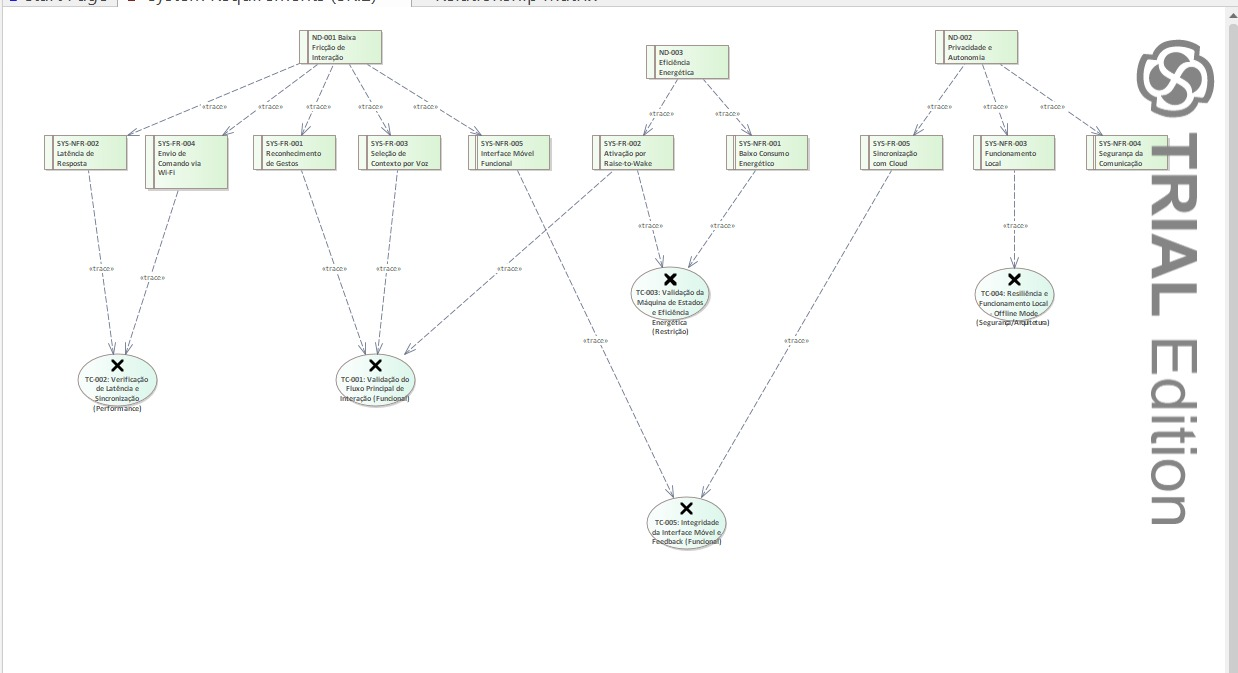
\includegraphics[width=0.95\textwidth]{e4_scheme.jpg}
    \caption{Protocolo de Testes (Test Protocol) modelado no Enterprise Architect.}
    \label{fig:e4_scheme}
\end{figure}

\begin{figure}[H]
    \centering
    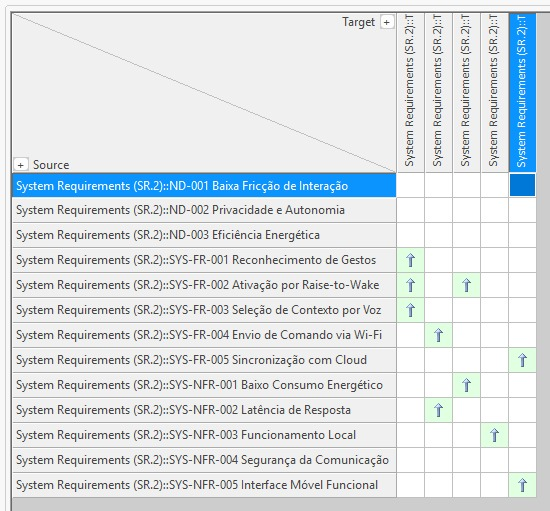
\includegraphics[width=0.65\textwidth]{test_matrix.jpg}
    \caption{Matriz de Rastreabilidade entre Requisitos de Sistema e Casos de Teste.}
    \label{fig:test_matrix}
\end{figure}

\clearpage

\section{System Architecture Design (E5)}

A arquitetura do sistema OmniBand foi desenhada com o objetivo de gerir a complexidade do projeto através da sua decomposição em blocos funcionais e físicos. A modelação foi realizada recorrendo à ferramenta Enterprise Architect e à linguagem SysML 1.5.

\subsection{Arquitetura Lógica e Física (Decomposição)}

A abstração inicial do sistema divide-o nas suas componentes principais. A Figura \ref{fig:bdd_omni} apresenta o Block Definition Diagram (BDD), que ilustra a estrutura hierárquica do sistema e a sua arquitetura física:

\begin{figure}[h!]
    \centering
    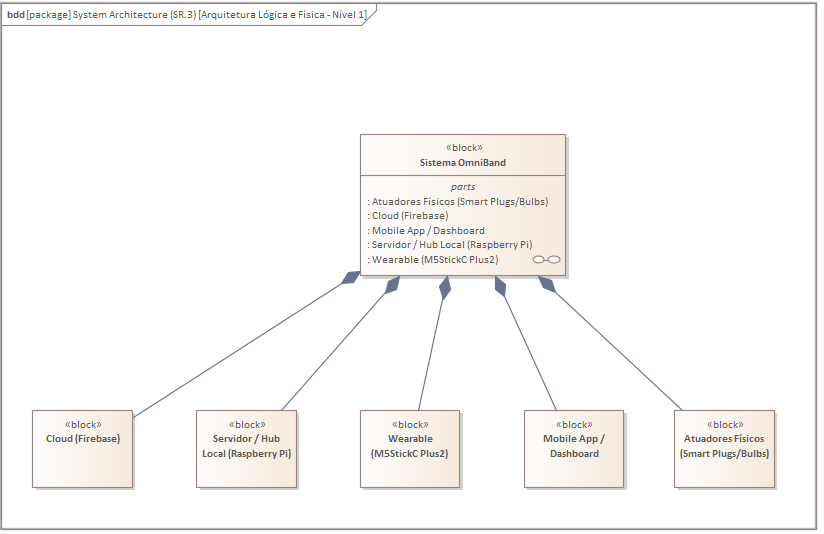
\includegraphics[width=0.9\textwidth]{E5_chart1.png}
    \caption{Block Definition Diagram (BDD) - Decomposição do Sistema OmniBand.}
    \label{fig:bdd_omni}
\end{figure}

\begin{itemize}
    \item \textbf{Wearable (Edge):} Implementado no microcontrolador M5CoreInk, com IMU BMI088 externo (acelerómetro + giroscópio) e microfone eletreto analógico. Atua como a unidade central de aquisição sensorial e de processamento local dos modelos TinyML para o reconhecimento de gestos.
    \item \textbf{Servidor / Hub Local:} Sustentado num Raspberry Pi com servidor Flask e Home Assistant. Funciona como o núcleo da rede local, traduzindo comandos e interagindo diretamente com os equipamentos residenciais.
    \item \textbf{Interfaces e Atuadores Externos:} O ecossistema é complementado pelo Dashboard Web (HTML/CSS/JS com polling AJAX), pela base de dados SQLite para persistência de eventos, e pelos Atuadores Físicos (Tomadas Tapo P110) que materializam a automação.
\end{itemize}

\subsection{Comunicações Internas e Fluxos de Dados}

Para garantir a baixa fricção e a baixa latência exigidas pelas necessidades dos stakeholders (ND-001 e ND-002), o modelo de comunicações foi otimizado. A Figura \ref{fig:ibd_omni} detalha as interfaces técnicas e o wiring interno do ecossistema através de um Internal Block Diagram (IBD).

\begin{figure}[h!]
    \centering
    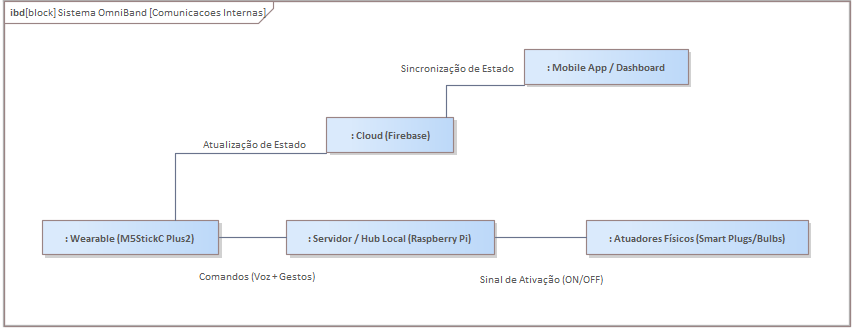
\includegraphics[width=0.9\textwidth]{E5_chart2.png}
    \caption{Internal Block Diagram (IBD) - Comunicações e Fluxos de Dados Internos.}
    \label{fig:ibd_omni}
\end{figure}

O Wearable emite os comandos processados localmente via Wi-Fi diretamente para o servidor Flask, que por sua vez aciona o Home Assistant para controlar os atuadores. Em paralelo, o Dashboard Web faz polling a cada 2 segundos para obter o estado atualizado dos dispositivos e o histórico de eventos.

\subsection{Máquina de Estados do Firmware}

O firmware do OmniBand implementa uma máquina de estados com 4 estados principais, otimizada para eficiência energética:

\begin{itemize}
    \item \textbf{IDLE:} Estado de repouso. O IMU é lido periodicamente. Se for detetado um movimento brusco (aceleração delta $>$ 3.0 m/s² ou velocidade angular $>$ 150 dps), o sistema transita para CONTEXT. Em paralelo, gestos simples por threshold (az $>$ 6.0 m/s² para cima, az $<$ -6.0 m/s² para baixo) são enviados diretamente ao servidor sem necessidade de contexto.
    \item \textbf{CONTEXT:} O microfone é ativado para deteção de palmas. O sistema conta palmas com debounce (200ms), gap máximo entre palmas (2.5s) e janela total de contexto (7s). 1 palma = corredor, 2 = sala, 3 = quarto. Após contexto definido, transita para GESTURE.
    \item \textbf{GESTURE:} O ecrã mostra ``PREPARA...'' (1s) e depois ``JÁ!'' (1s de recolha de dados IMU a 100Hz). Os 6 eixos (ax, ay, az, gx, gy, gz) são passados ao classificador Edge Impulse. Se o resultado for ``parado'', o ciclo repete. Se for ``cima'' ou ``baixo'', o comando é enviado ao servidor e o sistema transita para RESULT.
    \item \textbf{RESULT:} O ecrã mostra o resultado do comando (enviado/falhou) com o contexto, gesto e confiança. Após 5 segundos, retorna a IDLE.
\end{itemize}

\subsection{Algoritmo de Deteção Adaptativa de Palmas}

O sistema de deteção de palmas utiliza um algoritmo de limiar adaptativo com média exponencial móvel:

\begin{itemize}
    \item O noise floor é atualizado continuamente: $\text{noiseFloor} = \alpha \times \text{peakToPeak} + (1 - \alpha) \times \text{noiseFloor}$
    \item $\alpha = 0.12$ para subidas (resposta rápida a aumentos de ruído) e $\alpha = 0.025$ para descidas (decai lentamente)
    \item O limiar de deteção é: $\text{threshold} = \max(600, \text{noiseFloor} \times 2.8)$
    \item Uma palma é confirmada quando $\text{peakToPeak} \geq \text{threshold}$ e a leitura não é suspeita (média entre 30 e 3900)
\end{itemize}

\subsection{Modelo de Machine Learning (Edge Impulse)}

O modelo foi treinado na plataforma Edge Impulse com as seguintes características:

\begin{itemize}
    \item \textbf{Classes:} 3 — cima, baixo, parado
    \item \textbf{Sensor:} IMU (acelerómetro + giroscópio), 6 eixos
    \item \textbf{Janela temporal:} 1 segundo a 100 Hz (600 amostras totais)
    \item \textbf{Pré-processamento:} Spectral features (Edge Impulse DSP block)
    \item \textbf{Classificador:} Rede neuronal fully-connected (TFLite)
    \item \textbf{Inferência:} Local no microcontrolador, sem necessidade de cloud
\end{itemize}

O modelo foi exportado como biblioteca Arduino e integrado no firmware através do header \texttt{correia\_2k-project-1\_inferencing.h}.

\subsection{Características Físicas e Visuais da Solução}

\begin{itemize}
    \item \textbf{Físico (Wearable):} O microcontrolador M5CoreInk é acoplado ao pulso do utilizador através de uma bracelete. O IMU BMI088 é ligado externamente via I2C (pinos 32/33). O microfone eletreto é ligado ao pino analógico 36.
    \item \textbf{Visual (Interface E-Paper):} O ecrã de 200$\times$200 pixels apresenta:
    \begin{itemize}
        \item Ecrã IDLE: estado do WiFi, instruções de uso, botão de recalibração
        \item Ecrã CONTEXT: 3 caixas numeradas (1/2/3) que se preenchem à medida que as palmas são detetadas, limiar do microfone
        \item Ecrã GESTURE: contexto selecionado, opções CIMA/BAIXO, indicador de escuta animado (3 círculos progressivos)
        \item Ecrã RESULT: contexto, gesto detetado, confiança, estado do envio HTTP
    \end{itemize}
    \item \textbf{Visual (Web Dashboard):} Interface com sidebar de navegação, cards para adicionar gestos/dispositivos/regras, listas de gestos e dispositivos, estado dos dispositivos com botões ligar/desligar/toggle, e histórico de eventos com atualização automática a cada 2 segundos.
\end{itemize}

\subsection{Backend e Integração Home Assistant}

O servidor Flask expõe os seguintes endpoints principais:

\begin{itemize}
    \item \texttt{POST /api/trigger} — Recebe comandos do wearable (gesto, contexto, número de palmas) e executa as regras associadas
    \item \texttt{GET /api/devices} — Lista dispositivos com estado atual
    \item \texttt{POST /api/device/\{id\}/action} — Controla um dispositivo (on/off/toggle)
    \item \texttt{GET /api/logs} — Histórico de eventos
    \item \texttt{POST /api/ha/refresh} — Sincroniza estados com Home Assistant
\end{itemize}

A integração com Home Assistant é feita via REST API, utilizando um token de acesso de longa duração. O servidor consulta o estado real dos dispositivos no Home Assistant antes de executar ações, garantindo consistência.

\section{Conclusões (E6)}

O desenvolvimento do OmniBand ao longo do semestre demonstrou a viabilidade de construir um sistema de controlo residencial por gestos baseado em TinyML, mesmo perante condicionantes logísticas significativas. A indisponibilidade total do hardware planeado (M5StickC Plus2) e o atraso generalizado na entrega de materiais obrigaram a equipa a reformular a arquitetura do sistema em múltiplas frentes, pivotando para o M5CoreInk como plataforma principal.

\subsection{Principais Resultados Alcançados}

\begin{itemize}
    \item \textbf{Reconhecimento de Gestos com Edge Impulse:} Foi treinado e implementado com sucesso um modelo de Machine Learning capaz de classificar 3 gestos (cima, baixo, parado) diretamente no microcontrolador, utilizando dados do IMU BMI088 a 100 Hz. A inferência é feita localmente, sem dependência de cloud, garantindo privacidade e baixa latência.
    \item \textbf{Deteção Adaptativa de Palmas:} Desenvolveu-se um algoritmo de deteção de palmas com limiar adaptativo (média exponencial móvel) que permite selecionar contextos (corredor, sala, quarto) através de 1, 2 ou 3 palmas, contornando a limitação do microfone eletreto analógico que não permitia captação de voz.
    \item \textbf{Máquina de Estados Eficiente:} A máquina de estados com 4 fases (IDLE, CONTEXT, GESTURE, RESULT) otimiza o consumo energético ao ativar o microfone apenas quando necessário, após deteção de movimento do pulso (raise-to-wake).
    \item \textbf{Backend Local Integrado:} O servidor Flask no Raspberry Pi, integrado com Home Assistant, demonstra a capacidade de controlar dispositivos smart home reais (tomadas Tapo P110) a partir de comandos gestuais, com consistência de estado garantida por polling à API do Home Assistant.
    \item \textbf{Dashboard Web em Tempo Real:} A interface web desenvolvida permite configurar gestos, dispositivos e regras, visualizar o estado dos atuadores e consultar o histórico de eventos, com atualização automática a cada 2 segundos.
    \item \textbf{Interface E-Paper Otimizada:} O ecrã de tinta eletrónica do M5CoreInk foi explorado ao máximo, com modos de atualização rápida/lenta, animações incrementais (indicador de escuta) e desenho eficiente usando clip rects.
\end{itemize}

\subsection{Desafios e Lições Aprendidas}

O percurso do projeto evidenciou a importância da adaptabilidade em engenharia. A impossibilidade de utilizar o hardware previsto desde o início obrigou a repensar escolhas fundamentais:

\begin{itemize}
    \item A substituição do microfone MEMS (voz) por um eletreto analógico (apenas palmas) exigiu repensar o paradigma de interação, transformando a seleção de contexto de um ato de fala para um ato percussivo.
    \item A migração do M5StickC Plus2 para o M5CoreInk implicou a integração de sensores externos (BMI088) e a adaptação de toda a interface de utilizador para um ecrã e-paper de atualização lenta.
    \item A opção por um servidor local (Flask + Home Assistant) em vez de cloud (Firebase) revelou-se uma decisão acertada, proporcionando maior controlo sobre o sistema e eliminando dependências externas.
\end{itemize}

\subsection{Trabalho Futuro}

O protótipo atual estabelece as bases para várias direções de desenvolvimento futuro:

\begin{itemize}
    \item \textbf{Reconhecimento de Voz:} Com um microfone MEMS adequado, seria possível restaurar a interface de voz originalmente planeada, complementando as palmas com comandos vocais para contextos mais específicos.
    \item \textbf{Expansão do Vocabulário de Gestos:} O modelo Edge Impulse pode ser treinado com mais classes (ex.: círculo, swipe horizontal, shake) para suportar um leque mais alargado de comandos.
    \item \textbf{Modo Contínuo:} Implementar um modo de operação contínua onde o wearable monitoriza gestos sem necessidade de wake explícito, utilizando deteção de atividade (activity recognition) para filtrar movimentos relevantes.
    \item \textbf{Aplicação Móvel Nativa:} Desenvolver uma aplicação móvel nativa (Android/iOS) para substituir o dashboard web, oferecendo notificações push e integração com assistentes de voz do smartphone.
    \item \textbf{Otimização Energética:} Explorar modos de sleep profundo do ESP32 e comunicação BLE de baixo consumo para prolongar a autonomia da bateria.
\end{itemize}

\subsection{Considerações Finais}

O OmniBand cumpre o objetivo central do projeto: demonstrar que é possível construir um wearable de controlo residencial inteligente, baseado em TinyML, com processamento local e comunicação sem fios, utilizando hardware acessível e enfrentando condicionantes reais de engenharia. As adaptações realizadas ao longo do percurso não comprometeram a funcionalidade do sistema — pelo contrário, resultaram num protótipo robusto, com múltiplos modos de operação (gestos simples por threshold e gestos classificados por ML), integração com um ecossistema smart home real (Home Assistant) e uma interface web completa para configuração e monitorização.

O projeto demonstra que a combinação de Edge AI, wearables de baixo custo e automação residencial é uma via promissora para criar interfaces humano-máquina mais naturais, rápidas e privadas, aproximando-nos do conceito de ``varinha mágica'' que motivou este trabalho.

\end{document}
